\section{Electrode’s Kinetics}

We will now focus on the study of the kinetics of the electrochemical reactions happening on the electrodes boundaries. In particular, we will first start searching for a way to describe the transport of charge inside the system to then go into the mass transport phenomena. In this optics it will be quite useful to first recall some quantities that will be used inside the discussion.

Consider a general reduction reaction happening at an electrode, which can be written in the following form
\begin{equation}
    \ce{O + ne^-} \rightleftharpoons  \ce{R}.
\end{equation}
We will describe the rates at which a reaction take place by using the flux $\nu$ of electrons' moles that travels through the electrode surface. In this way we can describe also the current density on the surface by 
\begin{equation}
    J = nF\nu,
\end{equation}
where $n$ is the number of mole of electrons involved in the reduction reaction. Also, we know how both sides of the reaction are characterized by a transition rate $k_f$ and $k_b$ for the forward and backward direction, respectively. Such rates can be related to the flux easily by using the components surface density $C_i(x,t)$ and focus on the density at the surface as follows
\begin{align}
    &v_f = k_f C_O(0,t) = \frac{i_f}{nFA}, &v_b = k_b C_R(0,t) = \frac{i_b}{nFA},
\end{align}
where the surface was assumed to be at the position $x = 0$. If we connect this results we are already able to write down a form for the electrical current present in the system as
\begin{equation}
    \label{eq:TotalCurrentInterface}
    i = i_f - i_b = nFA[k_fC_O(0,t) - k_bC_R(0,t)].
\end{equation}
We only need to find a form for the quantities inside the equation, and that is basically what we are going to do in this section. 

Nevertheless, to be ready for that we shall also recall how we already know how $k$ can be computed by the use of transition state theory
\begin{equation}
    \label{eq:transitionRate}
    k = k_0\exp\left( -\frac{\Delta G^\ddagger}{RT} \right) = \kappa\frac{k_BT}{h}\exp\left( -\frac{\Delta G^\ddagger}{RT} \right).
\end{equation}
Where $\Delta G^\ddagger$ is the height of the barrier that separates the two states involved in the reaction, and the quantity $\kappa$ is called transmission coefficient expressing the probability to decay from the transition state to products.

\subsection{Butler-Volmer model}

To study the kinetics of electrons in the system we start from a standard condition of equilibrium in a one-electron single step reaction, which we approximate as in \figref{fig:ButlerVolmer}.
\begin{figure}[t]
    \centering
    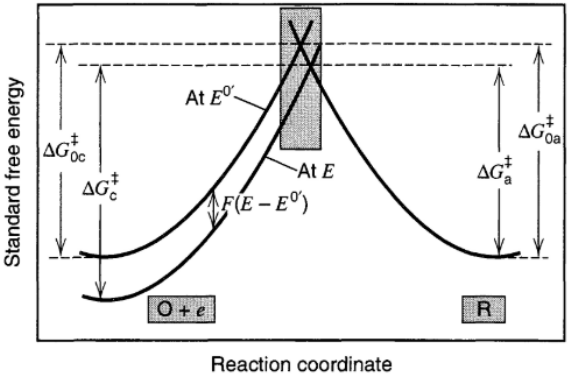
\includegraphics[width=0.45\textwidth]{Immagini/ButlerVolmer.png}
    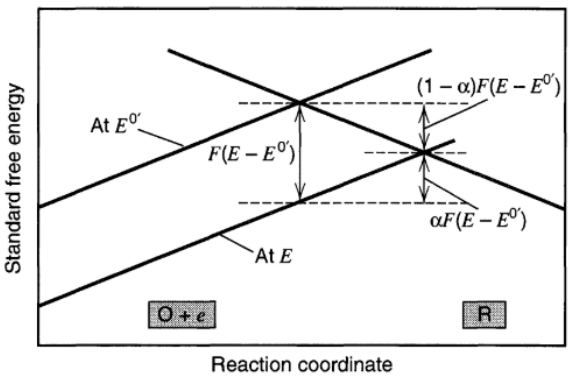
\includegraphics[width=0.45\textwidth]{Immagini/ButlerVolmer2.png}
    \caption{
        Approximation of the potential energy landscape inside a general reaction for some reaction coordinates. We are basically assuming that the reactants and products are minima in the energy and approximating the surrounding potential using second order Taylor expansion, so that the potential barrier is given by the interception of the parabolas.
    }
    \label{fig:ButlerVolmer}
\end{figure}
In that figure two conditions are depicted, a first one where we are in equilibrium so that the minima sits at the same height having so the same $\Delta G^\ddagger$ and therefore same rate, leading to $J = 0$. Then, we have the case where an external bias is applied and the energy of the electrons falls setting the reactants at lower potential generating a variation in the forward and backward barriers that can be estimated as follows
\begin{align*}
    &\Delta G_c^\ddagger = \Delta G_{0,c}^\ddagger - \alpha F(E - E^0), &\Delta G_a^\ddagger = \Delta G_{0,a}^\ddagger + (1 - \alpha) F(E - E^0).
\end{align*} 
Where $\alpha$ can be seen as an asymmetric factor, called transfer coefficient, that can range from zero to unity. Using these relations allows us to write down a form for the rates by inserting them inside \eqref{eq:transitionRate} to obtain
\begin{align}
    \label{eq:forwardRateC}
    &k_c = \kappa\frac{k_BT}{h}e^{-\frac{\Delta G^\ddagger_{0,c}}{RT}}\exp\left( -\frac{\alpha F(E-E^0)}{RT} \right), \\
    \label{eq:BackwardRateB}
    &k_a = \kappa\frac{k_BT}{h}e^{-\frac{\Delta G^\ddagger_{0,a}}{RT}}\exp\left( -\frac{(\alpha -1)F(E-E^0)}{RT} \right).
\end{align}
Knowing all of that we are able to obtain a really important result that is able to tell us the entity of the current inside our system as follows.
\thm{Butler-Volmer equation}
{
    The current flowing through the interface of an electrode, performing a general redox reaction, is given by the equation
    \begin{equation}
        i = FAk^0\left[ C_O(0,t)e^{-\alpha\frac{F(E - E^0)}{RT}} - C_R(0,t)e^{-(\alpha - 1)\frac{F(E-E^0)}{RT}} \right].
    \end{equation}
}
\pf{Proof}
{
    From \eqref{eq:forwardRateC} and \eqref{eq:BackwardRateB} we can see how, since the system was supposed to be in equilibrium without bias, meaning $E=E^0$, the rates have the properties of $k_c(E=0) = k_b(E=0)$. This brings us to write down that
    \begin{equation}
        k^0 = \kappa\frac{k_BT}{h}e^{-\frac{\Delta G^\ddagger_{0,c}}{RT}} = \kappa\frac{k_BT}{h}e^{-\frac{\Delta G^\ddagger_{0,a}}{RT}},
    \end{equation}
    which substituted back into the equation and inserted inside \eqref{eq:TotalCurrentInterface} gives the result.
}